\begin{figure}[h]
\centering
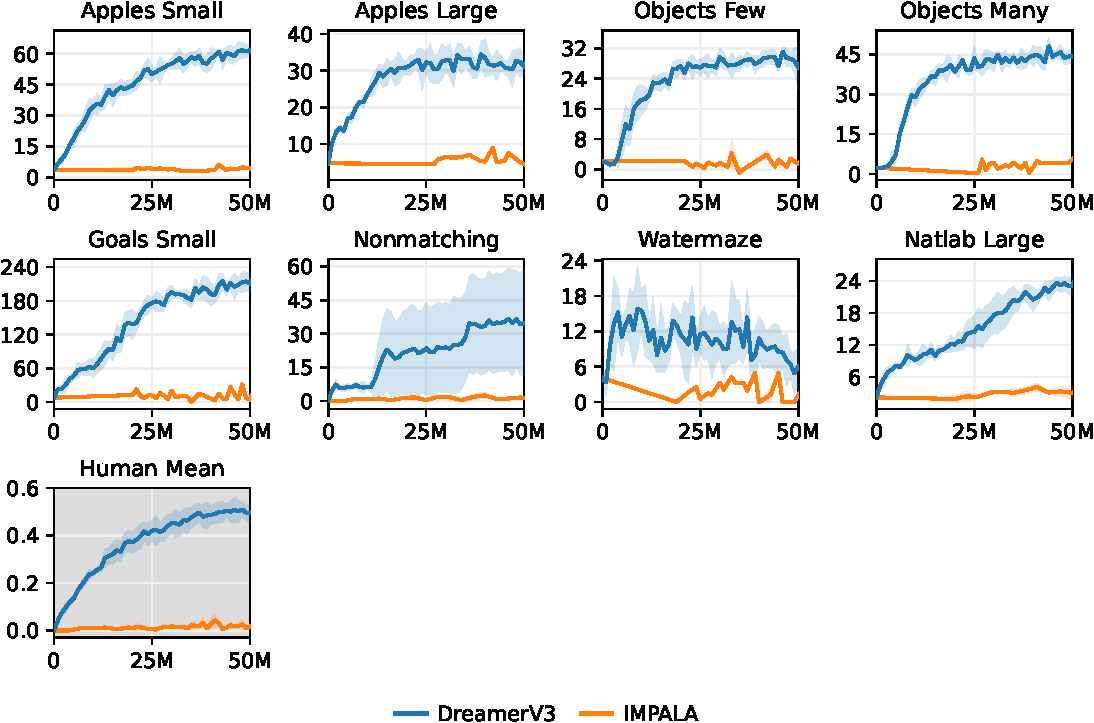
\includegraphics[width=1\linewidth]{dmlab/dmlab}
\caption{DMLab scores with a budget of 50M frames. Separate agents were trained for each task, corresponding to the IMPALA Experts method in \citet{espeholt2018impala}. Data efficiency is not the goal of IMPALA and it might be possible to tune it for improved data efficiency. Longer training curves and asymptotic performance of IMPALA are included in \cref{sec:dmlab_eff}.}
\label{fig:dmlab}
\end{figure}

\section*{DreamerV3}
\label{sec:method}

The DreamerV3 algorithm consists of 3 neural networks---the world model, the critic, and the actor---that are trained concurrently from replayed experience without sharing gradients, as shown in \cref{fig:model}.
To succeed across domains, these components need to accommodate different signal magnitudes and robustly balance terms in their objectives.
This is challenging as we are not only targeting similar tasks within the same domain but aim to learn across different domains with fixed hyperparameters.
This section first explains a simple transformation for predicting quantities of unknown orders of magnitude.
We then introduce the world model, critic, and actor and their robust learning objectives.
Specifically, we find that combining KL balancing and free bits enables the world model to learn without tuning, and scaling down large returns without amplifying small returns allows a fixed policy entropy regularizer.
The differences to DreamerV2 are detailed in \cref{sec:diff}.

\subsection*{Symlog Predictions}

Reconstructing inputs and predicting rewards and values can be challenging because their scale can vary across domains.
Predicting large targets using a squared loss can lead to divergence whereas absolute and Huber losses \citep{mnih2015dqn} stagnate learning.
On the other hand, normalizing targets based on running statistics \citep{schulman2017ppo} introduces non-stationarity into the optimization.
We suggest \emph{symlog predictions} as a simple solution to this dilemma.
For this, a neural network $f(x,\theta)$ with inputs $x$ and parameters $\theta$ learns to predict a transformed version of its targets $y$.
To read out predictions $\hat{y}$ of the network, we apply the inverse transformation:

\eq{
\mathcal{L(\theta)} \doteq \textstyle\frac{1}{2}\big(f(x,\theta)-\symlog(y)\big)^2 \qquad
\hat{y} \doteq \symexp\!\big(f(x,\theta)\big)
\label{eq:logpred}}

As shown in \cref{fig:symlog}, using the logarithm as transformation would not allow us to predict targets that take on negative values.
Therefore, we choose a function from the bi-symmetric logarithmic family \citep{webber2012symlog} that we name \emph{symlog} as the transformation with the \emph{symexp} function as its inverse:

\eq{
\symlog(x) \doteq \sign(x)\ln\!\big(|x|+1\big) \qquad
\symexp(x) \doteq \sign(x)\big(\!\exp(|x|)-1\big)
\label{eq:symlog}}

\begin{figure}[h]
\centering
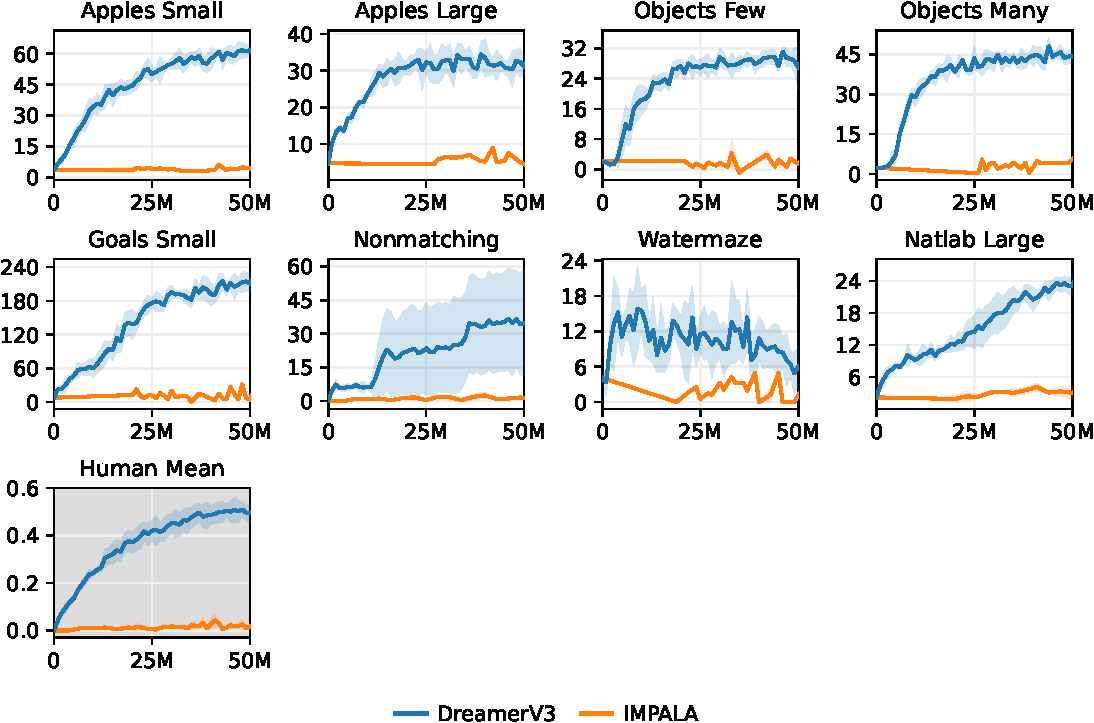
\includegraphics[width=1\linewidth]{dmlab/dmlab}
\caption{DMLab scores with a budget of 50M frames. Separate agents were trained for each task, corresponding to the IMPALA Experts method in \citet{espeholt2018impala}. Data efficiency is not the goal of IMPALA and it might be possible to tune it for improved data efficiency. Longer training curves and asymptotic performance of IMPALA are included in \cref{sec:dmlab_eff}.}
\label{fig:dmlab}
\end{figure}%
The symlog function compresses the magnitudes of both large positive and negative values.
Unlike the logarithm, it is symmetric around the origin while preserving the input sign.
This allows the optimization process to quickly move the network predictions to large values when needed.
Symlog approximates the identity around the origin so that it does not affect learning of targets that are already small enough.
For critic learning, a more involved transformation has previously been proposed \citep{kapturowski2018r2d2}, which we found less effective on average across domains.

DreamerV3 uses symlog predictions in the decoder, the reward predictor, and the critic. It
also squashes inputs to the encoder using the symlog function.
Despite its simplicity, this approach robustly and quickly learns across a diverse range of environments.
With symlog predictions, there is no need for truncating large rewards \citep{mnih2015dqn}, introducing non-stationary through reward normalization \citep{schulman2017ppo}, or adjusting network weights when new extreme values are detected \citep{hessel2019popart}.

\subsection*{World Model Learning}

The world model learns compact representations of sensory inputs through autoencoding \citep{hinton2006ae,kingma2013vae} and enables planning by predicting future representations and rewards for potential actions.
We implement the world model as a Recurrent State-Space Model (RSSM) \citep{hafner2018planet}, as shown in \cref{fig:model}.
First, an encoder maps sensory inputs $x_t$ to stochastic representations $z_t$.
Then, a sequence model with recurrent state $h_t$ predicts the sequence of these representations given past actions $a_{t-1}$.
The concatenation of $h_t$ and $z_t$ forms the model state from which we predict rewards $r_t$ and episode continuation flags $c_t\in\{0,1\}$ and reconstruct the inputs to ensure informative representations:

\eq{
\begin{alignedat}{4}
\raisebox{1.95ex}{\llap{\blap{\ensuremath{
\text{RSSM} \hspace{1ex} \begin{cases} \hphantom{A} \\ \hphantom{A} \\ \hphantom{A} \end{cases} \hspace*{-2.4ex}
}}}}
& \text{Sequence model:}        \padspace && h_t            &\ =    &\ f_\phi(h_{t-1},z_{t-1},a_{t-1}) \\
& \text{Encoder:}   \padspace && z_t            &\ \sim &\ \qp(z_t | h_t,x_t) \\
& \text{Dynamics predictor:}   \padspace && \hat{z}_t      &\ \sim &\ \pp(\hat{z}_t | h_t) \\
& \text{Reward predictor:}       \padspace && \hat{r}_t      &\ \sim &\ \pp(\hat{r}_t | h_t,z_t) \\
& \text{Continue predictor:}     \padspace && \hat{c}_t      &\ \sim &\ \pp(\hat{c}_t | h_t,z_t) \\
& \text{Decoder:}        \padspace && \hat{x}_t      &\ \sim &\ \pp(\hat{x}_t | h_t,z_t)
\end{alignedat}}

\Cref{fig:openl} visualizes long-term video predictions of the world world.
The encoder and decoder use convolutional neural networks (CNN) \citep{lecun1989cnn} for visual inputs and multi-layer perceptrons (MLPs) for low-dimensional inputs.
The dynamics, reward, and continue predictors are also MLPs.
The representations are sampled from a vector of softmax distributions and we take straight-through gradients through the sampling step \citep{bengio2013straight,hafner2020dreamerv2}.
Given a sequence batch of inputs $x_{1:T}$, actions $a_{1:T}$, rewards $r_{1:T}$, and continuation flags $c_{1:T}$, the world model parameters $\phi$ are optimized end-to-end to minimize the prediction loss $\mathcal{L}_{\mathrm{pred}}$, the dynamics loss $\mathcal{L}_{\mathrm{dyn}}$, and the representation loss $\mathcal{L}_{\mathrm{rep}}$ with corresponding loss weights $\beta_{\mathrm{pred}}=1$,  $\beta_{\mathrm{dyn}}=0.5$, $\beta_{\mathrm{rep}}=0.1$:

\eq{
\mathcal{L}(\phi)\doteq
\E_{q_\phi}<\Big>[\textstyle\sum_{t=1}^T(
    \beta_{\mathrm{pred}}\mathcal{L}_{\mathrm{pred}}(\phi)
   +\beta_{\mathrm{dyn}}\mathcal{L}_{\mathrm{dyn}}(\phi)
   +\beta_{\mathrm{rep}}\mathcal{L}_{\mathrm{rep}}(\phi)
)].
\label{eq:wm}
}

\begin{figure}[h]
\centering
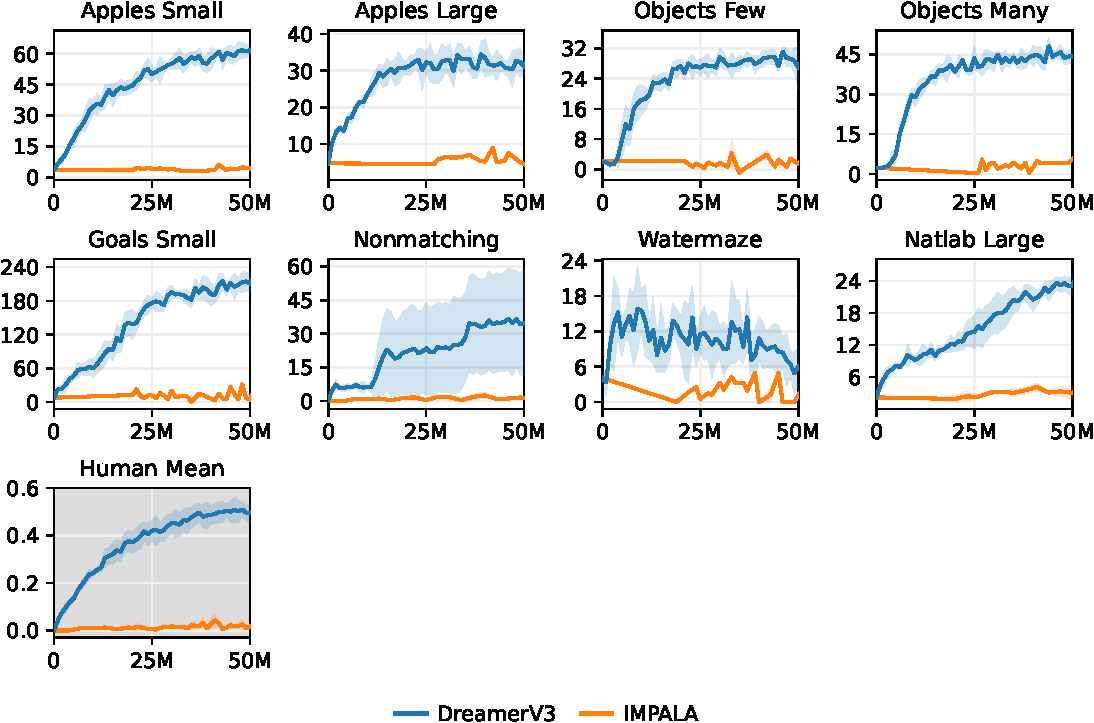
\includegraphics[width=1\linewidth]{dmlab/dmlab}
\caption{DMLab scores with a budget of 50M frames. Separate agents were trained for each task, corresponding to the IMPALA Experts method in \citet{espeholt2018impala}. Data efficiency is not the goal of IMPALA and it might be possible to tune it for improved data efficiency. Longer training curves and asymptotic performance of IMPALA are included in \cref{sec:dmlab_eff}.}
\label{fig:dmlab}
\end{figure}
\vspace*{-3ex}

The prediction loss trains the decoder and reward predictor via the symlog loss and the continue predictor via binary classification loss.
The dynamics loss trains the sequence model to predict the next representation by minimizing the KL divergence between the predictor $\pp(z_t|h_t)$ and the next stochastic representation $\qp(z_t|h_t,x_t)$.
The representation loss trains the representations to become more predictable if the dynamics cannot predict their distribution, allowing us to use a factorized dynamics predictor for fast sampling when training the actor critic.
The two losses differ in the stop-gradient operator $\operatorname{sg}(\cdot)$ and their loss scale.
To avoid a degenerate solution where the dynamics are trivial to predict but contain not enough information about the inputs, we employ free bits\citep{kingma2016freebits} by clipping the dynamics and representation losses below the value of 1 nat $\approx$ 1.44 bits.
This disables them while they are already minimized well to focus the world model on its prediction loss:

% \eq{
% \mathcal{L_{\mathrm{pred}}}(\phi) & \doteq
% -\lnpp(x_t|z_t,h_t)
% -\lnpp(r_t|z_t,h_t)
% -\lnpp(c_t|z_t,h_t) \\
% \mathcal{L_{\mathrm{dyn}}}(\phi) & \doteq
% \max\bigl(1,\KL[\sg(\qp(z_t|h_t,x_t)) || \pp(z_t|h_t)]\bigr) \\
% \mathcal{L_{\mathrm{rep}}}(\phi) & \doteq
% \max\bigl(1,\KL[\qp(z_t|h_t,x_t) || \sg(\pp(z_t|h_t))]\bigr)
% }

\eq{
\mathcal{L_{\mathrm{pred}}}(\phi) & \doteq
-\lnpp(x_t|z_t,h_t)
-\lnpp(r_t|z_t,h_t)
-\lnpp(c_t|z_t,h_t) \\
\mathcal{L_{\mathrm{dyn}}}(\phi) & \doteq
\max\bigl(1,\KL[\sg(\qp(z_t|h_t,x_t)) || \hspace{3.2ex}\pp(z_t|h_t)\hphantom{)}]\bigr) \\
\mathcal{L_{\mathrm{rep}}}(\phi) & \doteq
\max\bigl(1,\KL[\hspace{3.2ex}\qp(z_t|h_t,x_t)\hphantom{)} || \sg(\pp(z_t|h_t))]\bigr)
}

Previous world models require scaling the representation loss differently based on the visual complexity of the environment.
Complex 3D environments contain details unnecessary for control and thus prompt a stronger regularizer to simplify the representations and make them more predictable.
In 2D games, the background is often static and individual pixels may matter for the task, requiring a weak regularizer to perceive fine details.
We find that combining free bits with a small scale for the representation loss resolve this dilemma, allowing for fixed hyperparameters across domains.
Moreover, symlog predictions for the decoder unify the gradient scale of the prediction loss across environments, further stabilizing the trade-off with the representation loss.

We occasionally observed spikes the in KL losses in earlier experiments, consistent with reports for deep variational autoencoders \citep{vahdat2020nvae,child2020vdvae}. To prevent this, we parameterize the categorical distributions of the encoder and dynamics predictor as mixtures of 1\% uniform and 99\% neural network output, making it impossible for them to become near deterministic and thus ensuring well-scaled KL losses. Further model details and hyperparameters are summarized in \cref{tab:hparams}.

\subsection*{Actor Critic Learning}

The actor and critic neural networks learn behaviors purely from abstract sequences predicted by the world model \citep{sutton1991dyna,ha2018worldmodels}.
During environment interaction, we select actions by sampling from the actor network without lookahead planning.
The actor and critic operate on model states $s_t \doteq \{h_t,z_t\}$ and thus benefit from the Markovian representations learned by the world model.
The actor aims to maximize the expected return $R_t \doteq \textstyle\sum_{\tau=0}^\infty \gamma^\tau r_{t+\tau}$ with a discount factor $\gamma=0.997$ for each model state.
To consider rewards beyond the prediction horizon $T=16$, the critic learns to predict the return of each state under the current actor behavior:

\eq{
&\text{Actor:}\quad
&& a_t \sim \p<\pi_\theta>(a_t|s_t) \\
&\text{Critic:}\quad
&& v_\psi(s_t) \approx \E_{p_\phi,\pi_\theta}[R_t]
\label{eq:ac}
}

Starting from representations of replayed inputs, the dynamics predictor and actor produce a sequence of
imagined model states $s_{1:T}$, actions $a_{1:T}$, rewards $r_{1:T}$, and continuation flags $c_{1:T}$. To estimate returns that consider rewards beyond the prediction horizon, we compute bootstrapped $\lambda$-returns that integrate the predicted rewards and values \citep{sutton2018rlbook,schulman2015gae}:

\eq{
R^\lambda_t \doteq r_t + \gamma c_t \Big(
  (1 - \lambda) v_\psi(s_{t+1}) +
  \lambda R^\lambda_{t+1}
\Big) \qquad
R^\lambda_T \doteq v_\psi(s_T)
\label{eq:lambda}
}

\paragraph{Critic Learning}
A simple choice for the critic loss function would be to regress the $\lambda$-returns via squared error or symlog predictions. However, the critic predicts the expected value of a potentially widespread return distribution, which can slow down learning. We choose a discrete regression approach for learning the critic based on \emph{twohot} encoded targets \citep{bellemare2017c51,schrittwieser2019muzero,imani2018distregression,van2019nonlinearbellman} that let the critic maintain and refine a distribution over potential returns. For this, we transform returns using the symlog function and discretize the resulting range into a sequence $B$ of $K=255$ equally spaced buckets $b_i$. The critic network outputs a softmax distribution $\p<p_\psi>(b_i|s_t)$ over the buckets and its output is formed as the expected bucket value under this distribution. Importantly, the critic can predict any continuous value in the interval because its expected bucket value can fall between the buckets:

\eq{
v_\psi(s_t)
\doteq \symexp(\E_{\p<p_\psi>(b_i|s_t)}[b_i])
= \symexp(\p<p_\psi>(\cdot|s_t)^T B) \qquad
B \doteq \begin{bmatrix} -20 & ... & +20 \end{bmatrix}
}

To train the critic, we symlog transform the targets $R^\lambda_t$ and then twohot encode them into a soft label for the softmax distribution produced by the critic. Twohot encoding is a generalization of onehot encoding to continuous values. It produces a vector of length $|B|$ where all elements are $0$ except for the two entries closest to the encoded continuous number, at positions $k$ and $k+1$. These two entries sum up to $1$, with more weight given to the entry that is closer to the encoded number:

\eq{
\operatorname{twohot}(x)_i
\doteq \begin{cases}
|b_{k+1} - x| \,/\, |b_{k+1} - b_k| &\text{ if } i=k \\
|b_{k\hphantom{+1}} - x| \,/\, |b_{k+1} - b_k| &\text{ if } i=k+1 \\
0 &\text{ else} \\
\end{cases} \qquad
k \doteq \sum_{j=1}^B \operatorname{\delta}(b_j < x)
}

Given twohot encoded targets $y_t = \sg(\twohot(\symlog(R^\lambda_t)))$, where $\sg(\cdot)$ stops the gradient, the critic minimizes the categorical cross entropy loss for classification with soft targets:

\eq{
\mathcal{L}_{\mathrm{critic}}(\psi) \doteq
\sum_{t=1}^T \E_{b_i \sim y_t}[-\p<\ln p_\psi>(b_i|s_t)]
=
-\sum_{t=1}^T y_t^T \p<\ln p_\psi>(\cdot|s_t)
}

We found discrete regression for the critic to accelerate learning especially in environments with sparse rewards, likely because of their bimodal reward and return distributions.
We use the same discrete regression approach for the reward predictor of the world model.

Because the critic regresses targets that depend on its own predictions, we stabilize learning by regularizing the critic towards predicting the outputs of an exponentially moving average of its own parameters.
This is similar to target networks used previously in reinforcement learning \citep{mnih2015dqn} but allows us to compute returns using the current critic network.
We further noticed that the randomly initialized reward predictor and critic networks at the start of training can result in large predicted rewards that can delay the onset of learning.
We initialize the output weights of the reward predictor and critic to zeros, which effectively alleviates the problem and accelerates early learning.

\paragraph{Actor Learning}
The actor network learns to choose actions that maximize returns while ensuring sufficient exploration through an entropy regularizer \citep{williams1991maxentreinforce}.
However, the scale of this regularizer heavily depends on the scale and frequency of rewards in the environment, which has been a challenge for previous algorithms \citep{haarnoja2018sac}.
Ideally, we would like the policy to explore quickly in the absence of nearby returns without sacrificing final performance under dense returns.

To stabilize the scale of returns, we normalize them using moving statistics.
For tasks with dense rewards, one can simply divide returns by their standard deviation, similar to previous work \citep{schulman2017ppo}.
However, when rewards are sparse, the return standard deviation is generally small and this approach would amplify the noise contained in near-zero returns, resulting in an overly deterministic policy that fails to explore.
Therefore, we propose propose to scale down large returns without scaling up small returns.
We implement this idea by dividing returns by their scale $S$, for which we discuss multiple choices below, but only if they exceed a minimum threshold of $1$.
This simple change is the key to allowing a single entropy scale $\eta=3\cdot10^{-4}$ across dense and sparse rewards:

\eq{
\mathcal{L}(\theta)\doteq
\textstyle\sum_{t=1}^T
\E_{\pi_\theta,p_\phi}[\sg(R^\lambda_t)/\max(1, S)]
-\,\eta\H[\p<\pi_\theta>(a_t|s_t)]
\label{eq:pg}
}

We follow DreamerV2 \citep{hafner2020dreamerv2} in estimating the gradient of the first term by stochastic backpropagation for continuous actions and by reinforce \citep{williams1992reinforce} for discrete actions. The gradient of the second term is computed in closed form.

In deterministic environments, we find that normalizing returns by their exponentially decaying standard deviation suffices.
However, for heavily randomized environments, the return distribution can be highly non-Gaussian and contain outliers of large returns caused by a small number of particularly easy episodes, leading to an overly deterministic policy that struggles to sufficiently explore.
To normalize returns while being robust to such outliers, we scale returns by an exponentially decaying average of the range from their
5\textsuperscript{th} to their 95\textsuperscript{th} batch percentile:

\eq{
S =
\operatorname{Per}(R^\lambda_t, 95) -
\operatorname{Per}(R^\lambda_t, 5)
}

Because a constant return offset does not affect the objective, this is equivalent to an affine transformation that maps these percentiles to $0$ and $1$, respectively.
Compared to advantage normalization \citep{schulman2017ppo}, scaling returns down accelerates exploration under sparse rewards without sacrificing final performance under dense rewards, while using a fixed entropy scale.
